% This contents of this file will be inserted into the _Solutions version of the
% output tex document.  Here's an example:

% If assignment with subquestion (1.a) requires a written response, you will
% find the following flag within this document: <SCPD_SUBMISSION_TAG>_1a
% In this example, you would insert the LaTeX for your solution to (1.a) between
% the <SCPD_SUBMISSION_TAG>_1a flags.  If you also constrain your answer between the
% START_CODE_HERE and END_CODE_HERE flags, your LaTeX will be styled as a
% solution within the final document.

% Please do not use the '<SCPD_SUBMISSION_TAG>' character anywhere within your code.  As expected,
% that will confuse the regular expressions we use to identify your solution.
\def\assignmentnum{1 }
\def\assignmenttitle{XCS229 Problem Set \assignmentnum}

\documentclass{article}
\usepackage[top = 1.0in]{geometry}

\usepackage{graphicx}

\usepackage[utf8]{inputenc}
\usepackage{listings}
\usepackage[dvipsnames]{xcolor}
\usepackage{bm}
\usepackage{algorithm}
\usepackage{algpseudocode}
\usepackage{framed}

\definecolor{codegreen}{rgb}{0,0.6,0}
\definecolor{codegray}{rgb}{0.5,0.5,0.5}
\definecolor{codepurple}{rgb}{0.58,0,0.82}
\definecolor{backcolour}{rgb}{0.95,0.95,0.92}

\lstdefinestyle{mystyle}{
    backgroundcolor=\color{backcolour},   
    commentstyle=\color{codegreen},
    keywordstyle=\color{magenta},
    stringstyle=\color{codepurple},
    basicstyle=\ttfamily\footnotesize,
    breakatwhitespace=false,         
    breaklines=true,                 
    captionpos=b,                    
    keepspaces=true,                 
    numbersep=5pt,                  
    showspaces=false,                
    showstringspaces=false,
    showtabs=false,                  
    tabsize=2
}

\lstset{style=mystyle}

\newcommand{\di}{{d}}
\newcommand{\nexp}{{n}}
\newcommand{\nf}{{p}}
\newcommand{\vcd}{{\textbf{D}}}
\newcommand{\Int}{\mathbb{Z}}
\newcommand\bb{\ensuremath{\mathbf{b}}}
\newcommand\bs{\ensuremath{\mathbf{s}}}
\newcommand\bp{\ensuremath{\mathbf{p}}}
\newcommand{\relu} { \operatorname{ReLU} }
\newcommand{\smx} { \operatorname{softmax} }
\newcommand\bx{\ensuremath{\mathbf{x}}}
\newcommand\bh{\ensuremath{\mathbf{h}}}
\newcommand\bc{\ensuremath{\mathbf{c}}}
\newcommand\bW{\ensuremath{\mathbf{W}}}
\newcommand\by{\ensuremath{\mathbf{y}}}
\newcommand\bo{\ensuremath{\mathbf{o}}}
\newcommand\be{\ensuremath{\mathbf{e}}}
\newcommand\ba{\ensuremath{\mathbf{a}}}
\newcommand\bu{\ensuremath{\mathbf{u}}}
\newcommand\bv{\ensuremath{\mathbf{v}}}
\newcommand\bP{\ensuremath{\mathbf{P}}}
\newcommand\bg{\ensuremath{\mathbf{g}}}
\newcommand\bX{\ensuremath{\mathbf{X}}}
% real numbers R symbol
\newcommand{\Real}{\mathbb{R}}

% encoder hidden
\newcommand{\henc}{\bh^{\text{enc}}}
\newcommand{\hencfw}[1]{\overrightarrow{\henc_{#1}}}
\newcommand{\hencbw}[1]{\overleftarrow{\henc_{#1}}}

% encoder cell
\newcommand{\cenc}{\bc^{\text{enc}}}
\newcommand{\cencfw}[1]{\overrightarrow{\cenc_{#1}}}
\newcommand{\cencbw}[1]{\overleftarrow{\cenc_{#1}}}

% decoder hidden
\newcommand{\hdec}{\bh^{\text{dec}}}

% decoder cell
\newcommand{\cdec}{\bc^{\text{dec}}}

\usepackage[hyperfootnotes=false]{hyperref}
\hypersetup{
  colorlinks=true,
  linkcolor = blue,
  urlcolor  = blue,
  citecolor = blue,
  anchorcolor = blue,
  pdfborderstyle={/S/U/W 1}
}
\usepackage{nccmath}
\usepackage{mathtools}
\usepackage{graphicx,caption}
\usepackage[shortlabels]{enumitem}
\usepackage{epstopdf,subcaption}
\usepackage{psfrag}
\usepackage{amsmath,amssymb,epsf}
\usepackage{verbatim}
\usepackage{cancel}
\usepackage{color,soul}
\usepackage{bbm}
\usepackage{listings}
\usepackage{setspace}
\usepackage{float}
\definecolor{Code}{rgb}{0,0,0}
\definecolor{Decorators}{rgb}{0.5,0.5,0.5}
\definecolor{Numbers}{rgb}{0.5,0,0}
\definecolor{MatchingBrackets}{rgb}{0.25,0.5,0.5}
\definecolor{Keywords}{rgb}{0,0,1}
\definecolor{self}{rgb}{0,0,0}
\definecolor{Strings}{rgb}{0,0.63,0}
\definecolor{Comments}{rgb}{0,0.63,1}
\definecolor{Backquotes}{rgb}{0,0,0}
\definecolor{Classname}{rgb}{0,0,0}
\definecolor{FunctionName}{rgb}{0,0,0}
\definecolor{Operators}{rgb}{0,0,0}
\definecolor{Background}{rgb}{0.98,0.98,0.98}
\lstdefinelanguage{Python}{
    numbers=left,
    numberstyle=\footnotesize,
    numbersep=1em,
    xleftmargin=1em,
    framextopmargin=2em,
    framexbottommargin=2em,
    showspaces=false,
    showtabs=false,
    showstringspaces=false,
    frame=l,
    tabsize=4,
    % Basic
    basicstyle=\ttfamily\footnotesize\setstretch{1},
    backgroundcolor=\color{Background},
    % Comments
    commentstyle=\color{Comments}\slshape,
    % Strings
    stringstyle=\color{Strings},
    morecomment=[s][\color{Strings}]{"""}{"""},
    morecomment=[s][\color{Strings}]{'''}{'''},
    % keywords
    morekeywords={import,from,class,def,for,while,if,is,in,elif,else,not,and,or
    ,print,break,continue,return,True,False,None,access,as,,del,except,exec
    ,finally,global,import,lambda,pass,print,raise,try,assert},
    keywordstyle={\color{Keywords}\bfseries},
    % additional keywords
    morekeywords={[2]@invariant},
    keywordstyle={[2]\color{Decorators}\slshape},
    emph={self},
    emphstyle={\color{self}\slshape},
%
}
\lstMakeShortInline|

\pagestyle{empty} \addtolength{\textwidth}{1.0in}
\addtolength{\textheight}{0.5in}
\addtolength{\oddsidemargin}{-0.5in}
\addtolength{\evensidemargin}{-0.5in}
\newcommand{\ruleskip}{\bigskip\hrule\bigskip}
\newcommand{\nodify}[1]{{\sc #1}}
\newenvironment{answer}{\sf \begingroup\color{ForestGreen}}{\endgroup}%

\setlist[itemize]{itemsep=2pt, topsep=0pt}
\setlist[enumerate]{itemsep=6pt, topsep=0pt}

\setlength{\parindent}{0pt}
\setlength{\parskip}{4pt}
\setlist[enumerate]{parsep=4pt}
\setlength{\unitlength}{1cm}

\renewcommand{\Re}{{\mathbb R}}
\newcommand{\R}{\mathbb{R}}
\newcommand{\what}[1]{\widehat{#1}}

\renewcommand{\comment}[1]{}
\newcommand{\mc}[1]{\mathcal{#1}}
\newcommand{\half}{\frac{1}{2}}

\DeclareMathOperator*{\argmin}{arg\,min}

\def\KL{D_{KL}}
\def\xsi{x^{(i)}}
\def\ysi{y^{(i)}}
\def\zsi{z^{(i)}}
\def\E{\mathbb{E}}
\def\calN{\mathcal{N}}
\def\calD{\mathcal{D}}
\def\slack{\url{http://xcs229-scpd.slack.com/}}
\def\zipscriptalt{\texttt{python zip\_submission.py}}
\DeclarePairedDelimiter\abs{\lvert}{\rvert}%
 
\usepackage{bbding}
\usepackage{pifont}
\usepackage{wasysym}
\usepackage{amssymb}
\usepackage{framed}
\usepackage{scrextend}

\newcommand{\alns}[1] {
	\begin{align*} #1 \end{align*}
}

\newcommand{\pd}[2] {
 \frac{\partial #1}{\partial #2}
}
\renewcommand{\Re} { \mathbb{R} }
\newcommand{\btx} { \mathbf{\tilde{x}} }
\newcommand{\bth} { \mathbf{\tilde{h}} }
\newcommand{\sigmoid} { \operatorname{\sigma} }
\newcommand{\CE} { \operatorname{CE} }
\newcommand{\byt} { \hat{\by} }
\newcommand{\yt} { \hat{y} }

\newcommand{\oft}[1]{^{(#1)}}
\newcommand{\fone}{\ensuremath{F_1}}

\newcommand{\ac}[1]{ {\color{red} \textbf{AC:} #1} }
\newcommand{\ner}[1]{\textbf{\color{blue} #1}}
\begin{document}
\pagestyle{myheadings} \markboth{}{\assignmenttitle}

% <SCPD_SUBMISSION_TAG>_entire_submission

This handout includes space for every question that requires a written response.
Please feel free to use it to handwrite your solutions (legibly, please).  If
you choose to typeset your solutions, the |README.md| for this assignment includes
instructions to regenerate this handout with your typeset \LaTeX{} solutions.
\ruleskip

\LARGE
1.a
\normalsize

% <SCPD_SUBMISSION_TAG>_1a
\begin{answer}
  % ### START CODE HERE ###
  Since
  \[
  \int\limits_{-\infty}^\infty{p(y;\eta)}{dy} = 1\newline
  \]
  then
  \[
  \frac{\partial}{\partial \eta} \int\limits_{-\infty}^\infty{p(y;\eta)} dy = \int\limits_{-\infty}^\infty \frac{\partial}{\partial \eta}{p(y;\eta)}{dy} = 0
  \]
  
  The probability mass function looks as follows:
  \[
  p(y;\eta) = b(y)e^{\eta y - a(\eta)}
  \]

  Its partial derivative with respect to $\eta$:
  \[
  \frac{\partial p(y;\eta)}{\partial \eta} = \frac{\partial}{\partial \eta} b(y) e^{\eta y - a(\eta)} = b(y)\frac{\partial}{\partial \eta} e^{\eta y - a(\eta)} = b(y) e^{\eta y - a(\eta)} (y - \frac{\partial a(\eta)}{\partial \eta} ) = p(y;\eta) (y - \frac{\partial a(\eta)}{\partial \eta} )
  \]

  Let's put it into the integral mentioned above:
  \[
  \int\limits_{-\infty}^\infty \frac{\partial}{\partial \eta}{p(y;\eta)}{dy} = \int\limits_{-\infty}^\infty{p(y;\eta) (y - \frac{\partial a(\eta)}{\partial \eta} )} dy = \int\limits_{-\infty}^\infty{p(y;\eta)} ydy - \int\limits_{-\infty}^\infty{ \frac{\partial a(\eta)}{\partial \eta}} dy
  \]

  since the first part is an expectation and $a(\eta)$ does not depend on y, then

  \[
  \int\limits_{-\infty}^\infty{p(y;\eta)} ydy - \int\limits_{-\infty}^\infty{ \frac{\partial a(\eta)}{\partial \eta}} dy = \mathbb{E} [Y;\eta] - \frac{\partial a(\eta)}{\partial \eta} = 0
  \]

  therefore
  \[
  \mathbb{E} [Y;\eta] = \frac{\partial a(\eta)}{\partial \eta}
  \]
  % ### END CODE HERE ###
\end{answer}
% <SCPD_SUBMISSION_TAG>_1a
\clearpage

\LARGE
1.b
\normalsize

% <SCPD_SUBMISSION_TAG>_1b
\begin{answer}
  % ### START CODE HERE ###
  Let us recall the following:
\[   \frac{\partial}{\partial \eta} \int\limits_{-\infty}^\infty{p(y;\eta)} dy = \int\limits_{-\infty}^\infty \frac{\partial}{\partial \eta}{p(y;\eta)}{dy} = 0   \]
  This is also valid: \[
  \frac{\partial^2}{\partial \eta^2} \int\limits_{-\infty}^\infty{p(y;\eta)} dy = \int\limits_{-\infty}^\infty \frac{\partial^2}{\partial \eta^2}{p(y;\eta)}{dy} = 0
  \]

  From the previous task we know that:
\[   \frac{\partial p(y;\eta)}{\partial \eta} = p(y;\eta) (y - \frac{\partial a(\eta)}{\partial \eta} )   \]

  Let us calculate the second derivative of $p$ with respect to $\eta$:
  \[
  \frac{\partial^2}{\partial \eta^2}{p(y;\eta)} = \frac{\partial}{\partial \eta} (p(y;\eta) (y - \frac{\partial a(\eta)}{\partial \eta} )) = (y - \frac{\partial a(\eta)}{\partial \eta})\frac{\partial p(y;\eta)}{\partial \eta} - p(y;\eta)\frac{\partial^2 a(\eta)}{\partial \eta^2} = (y - \frac{\partial a(\eta)}{\partial \eta})^2 p(y;\eta) - p(y;\eta)\frac{\partial^2 a(\eta)}{\partial \eta^2} 
  \]

  Therefore:
  \[
  \int\limits_{-\infty}^\infty \frac{\partial^2}{\partial \eta^2}{p(y;\eta)}{dy} = 
  \int\limits_{-\infty}^\infty (y - \frac{\partial a(\eta)}{\partial \eta})^2 p(y;\eta) - p(y;\eta)\frac{\partial^2 a(\eta)}{\partial \eta^2} {dy} = 0
  \]

  and
  \[
  \int\limits_{-\infty}^\infty (y - \frac{\partial a(\eta)}{\partial \eta})^2 p(y;\eta){dy} = \int\limits_{-\infty}^\infty p(y;\eta)\frac{\partial^2 a(\eta)}{\partial \eta^2} {dy} = \frac{\partial^2 a(\eta)}{\partial \eta^2}
  \]

  since we know that $\mathbb{E} [Y;\eta] = \frac{\partial a(\eta)}{\partial \eta}$, then let's rewrite the expression above taking this into account:
  \[
  \int\limits_{-\infty}^\infty (y - \mathbb{E}[Y;\eta])^2 p(y;\eta){dy} =  \frac{\partial^2 a(\eta)}{\partial \eta^2}
  \]

  The integral is actually variance, since by definition:
  \[
  Var[Y] = \mathbb{E}[(Y-\mathbb{E}[Y])^2]
  \]

  Therefore:
  \[
  Var[Y;\eta] = \frac{\partial^2 a(\eta)}{\partial \eta^2}
  \]
  % ### END CODE HERE ###
\end{answer}
% <SCPD_SUBMISSION_TAG>_1b
\clearpage

\LARGE
1.c
\normalsize

% <SCPD_SUBMISSION_TAG>_1c
\begin{answer}
  % ### START CODE HERE ###
  Starting with that probability mass function looks as follows:
  \[
  p(y;\eta) = b(y)e^{\eta y - a(\eta)}
  \]

  For $x_i$, $y_i$ and $\eta_i=\theta^Tx_i$ the likelihood will be: \[
\log p(y_i \mid \eta_i) = \log p(y_i \mid x_i; \theta) = \log b(y_i) + \eta_i y_i - a(\eta_i)
\]

Since $b(y_i)$ is independent from $\theta$, the negative log loss:
\[
\ell(\theta) = \sum_{i=1}^{n} \left[ a(\theta^\top x_i) - y_i \, \theta^\top x_i \right]
\]

The gradient:
\[
\nabla_\theta \ell(\theta) = \sum_{i=1}^{n} \left( \frac{da(\eta_i)}{d \theta} x_i - y_i x_i \right)
= \sum_{i=1}^{n} \left( \frac{da(\eta_i)}{d\eta_i}\frac{d\eta_i}{d\theta} - y_i x_i \right) = \sum_{i=1}^{n} \left( \frac{d a(\eta_i)}{d \eta_i} - y_i \right) x_i
\]

The Hessian:
\[
\nabla^2_\theta \ell(\theta) = \sum_{i=1}^{n} \frac{d^2 a(\eta_i)}{d \eta_i^2} \, x_i x_i^\top
\]

we know from reasoning in the previous tasks that $\frac{d^2 a(\eta_i)}{d\eta_i^2}$ is variance and it's a non-negative value. $x_i x_i^\top$ is always PSD because for any vector $z \in \mathbb{R}^d$

\[
z^\top (x_i x_i^\top) z = (z^\top x_i)(x_i^\top z) = (x_i^\top z)^2 \geq 0
\]

Therefore 
\[
\nabla^2_\theta \ell(\theta) = \sum_{i=1}^{n} \frac{d^2 a(\eta_i)}{d \eta_i^2} \, x_i x_i^\top \geq 0
\]
  % ### END CODE HERE ###
\end{answer}
% <SCPD_SUBMISSION_TAG>_1c
\clearpage

\LARGE
2.a
\normalsize

% <SCPD_SUBMISSION_TAG>_2a
\begin{answer}
  
  \begin{align*}
      % ### START CODE HERE ###
      J(\theta) = \frac{1}{2n} \sum_{i=1}^{n} \left( h_\theta (\hat{x}^{(i)}) - y^{(i)} \right)^2 = \frac{1}{2n} \sum_{i=1}^{n} \left( \theta^T \hat{x}^{(i)} - y^{(i)} \right)^2
      % ### END CODE HERE ###
  \end{align*}

  Differentiating this objective, we get:
  \begin{align*}
      % ### START CODE HERE ###
      \nabla_{\theta} J(\theta) = \frac{1}{n} \sum_{i=1}^{n} \left( \theta^T \hat{x}^{(i)} - y^{(i)} \right) \hat{x}^{(i)}
      % ### END CODE HERE ###
  \end{align*}
  % ### START CODE HERE ###
  % ### END CODE HERE ###
  The gradient descent update rule is
  %
  \begin{equation*}
  \theta := \theta - \lambda \nabla_{\theta} J(\theta)
  \end{equation*}
  %
  which reduces here to:
  % ### START CODE HERE ###
  \[
  \theta := \theta - \frac{\lambda}{n} \sum_{i=1}^{n} \left( \theta^T \hat{x}^{(i)} - y^{(i)} \right) \hat{x}^{(i)}
  \]
  % ### END CODE HERE ###
\end{answer}
% <SCPD_SUBMISSION_TAG>_2a
\clearpage

\LARGE
2.c
\normalsize

% <SCPD_SUBMISSION_TAG>_2c
\begin{answer}
  % ### START CODE HERE ###
  For value k=1 the regression becomes the line $1 + \theta_1 x$. It is underfitting.
  
  For value k=2 the regression becomes the function $1 + \theta_1 x + \theta_2 x^2$. Here we can see that the line is almost the same as the function above. This means that the calculated value of $\theta_2$ is small compared to $\theta_1$. The loss function is comparable with the function above. The regression underfits.

  For value k=3 the regression contains cubic components and is still underfitting, but starts to fit better due to presence of cubic component.

  For value k=5 and k=10 it seems the regression has the best fit and generalizes well.

  For value k=20 the regression is overfitting and starts catching the fluctuations of input data.
  % ### END CODE HERE ###
\end{answer}
% <SCPD_SUBMISSION_TAG>_2c
\clearpage

\LARGE
2.e
\normalsize

% <SCPD_SUBMISSION_TAG>_2e
\begin{answer}
  % ### START CODE HERE ###
  For values k=1, 2, 3, 5 the regression fits well.
  For value k=10 the regression has the best fit.
  For value k=20 the regression is overfitting and starts catching the fluctuations of input data.

  The difference is that the fitted model is different and the sinusoid function is used instead of polynome. The sinusoid fits better from the start compared to polynome.
  % ### END CODE HERE ###
\end{answer}
% <SCPD_SUBMISSION_TAG>_2e
\clearpage

\LARGE
2.g
\normalsize

% <SCPD_SUBMISSION_TAG>_2g
\begin{answer}
  % ### START CODE HERE ###
  There is lack of input points, however, the logic remains the same - for k=1,2,3 we see that the polynome line is not going through the points and not fitting well. For k = 5 it fits the best and for higher values it's overfitting. Definitely it's required to add more data for the model to predict better. Otherwise, the model will perform well on training and much worse on test data.

  For sinusoidal function it goes a bit better from the start but starts to overfit from k=5.
  % ### END CODE HERE ###
\end{answer}
% <SCPD_SUBMISSION_TAG>_2g
\clearpage

\LARGE
3.a
\normalsize

% <SCPD_SUBMISSION_TAG>_3a
\begin{answer}
  % ### START CODE HERE ###
  In A dataset the data for y=1.0 and y=0.0 is overlapping on x0, x1 scale. It means that there is a zone in x0, x1 plane where the points have randomly y=1.0 and y=0.0 values.

  The highest difference is that regression doesn't converge that quick on dataset B as it converges on dataset A.  
  % ### END CODE HERE ###
\end{answer}
\begin{figure}
  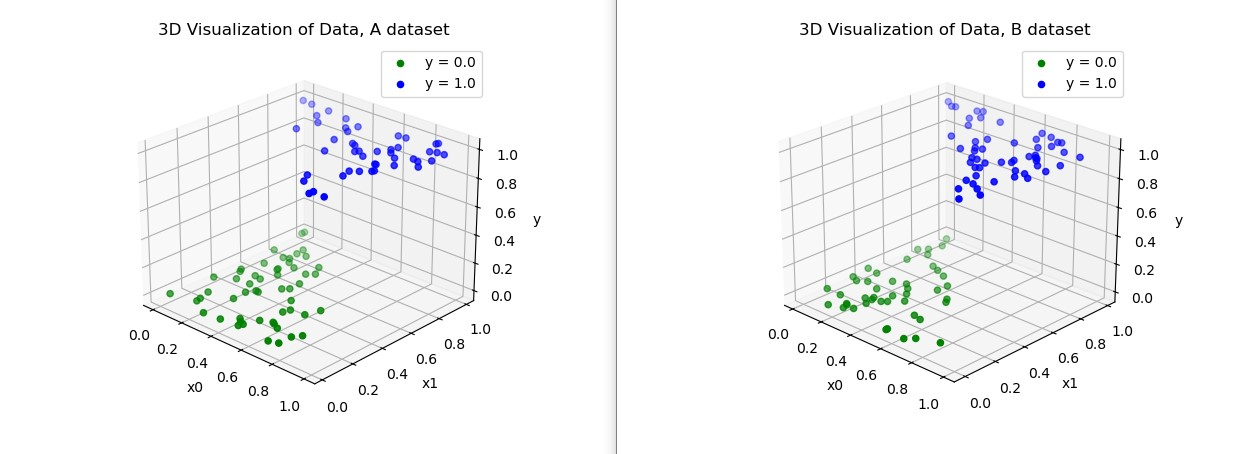
\includegraphics[width=\linewidth]{a_vs_b_dataset.jpg}
  \caption{A vs B dataset}
  \label{fig:avsb}
\end{figure}
\begin{figure}
  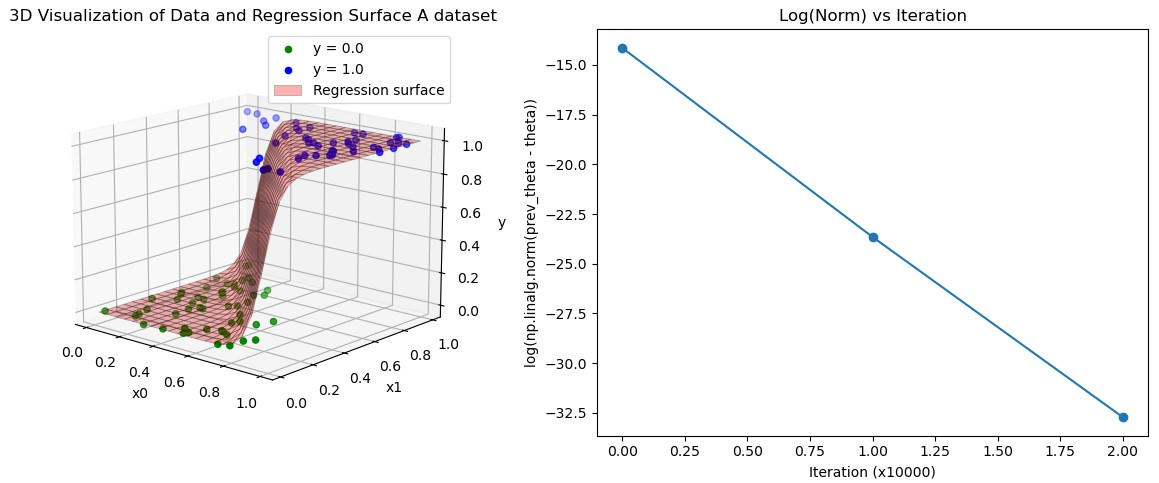
\includegraphics[width=\linewidth]{a_dataset_plots.jpg}
  \caption{Dataset A}
  \label{fig:a_dataset}
\end{figure}

\begin{figure}
  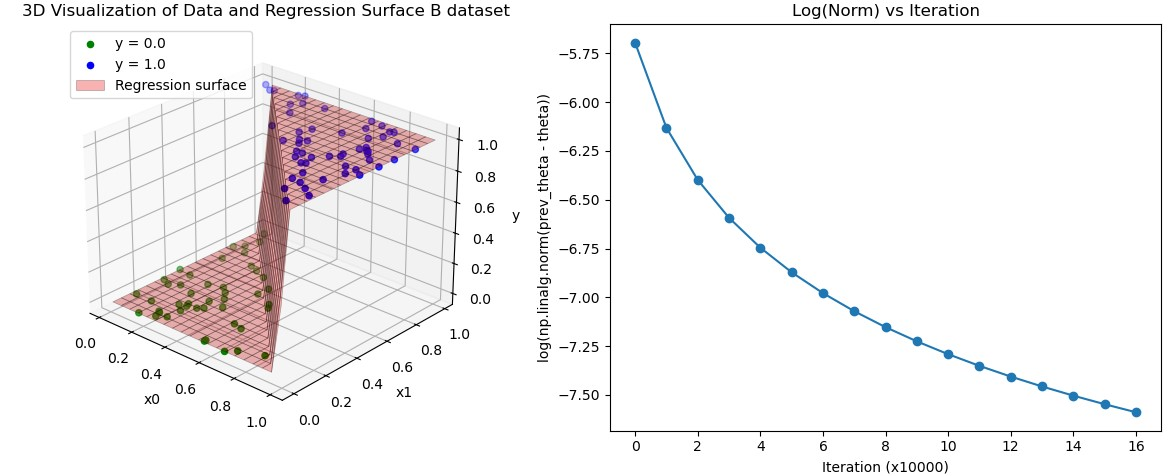
\includegraphics[width=\linewidth]{b_dataset_plots.jpg}
  \caption{Dataset B}
  \label{fig:a_dataset}
\end{figure}
% <SCPD_SUBMISSION_TAG>_3a

\LARGE
3.b
\normalsize

% <SCPD_SUBMISSION_TAG>_3b
\begin{answer}
  % ### START CODE HERE ###
  The specifics of the dataset A implies some fluctuation of the points, that do not allow the loss function to closely adapt to the points. Finally, the change of the loss function becomes negligible with respect to iteration. See figure 2.

  For dataset A:\newline
  Theta 10K iterations: [-20.81394174  21.45250215  19.85155266]\newline
  Theta 20K iterations: [-20.81437785  21.45295156  19.85198173]\newline
  Theta 30K iterations: [-20.81437788  21.45295159  19.85198176]\newline

  Dataset B is clearly separable. On dataset B the model catches well the separation. However $\theta$ parameter increases to really high values, due to the specifics of dataset B. This leads to situation, when each new calculated value of vector of $\theta$ values hugely differs from the previous value. Each module of $\theta$ is higher than the previous one. Nevertheless, the regression converges, but very slowly - see figure 3.

  For dataset B:\newline
  Theta 140K iterations: [-136.0833065   136.45725847  136.09754179]\newline
  Theta 150K iterations: [-139.33136783  139.73026941  139.34109305]\newline
  Theta 160K iterations: [-142.43475235  142.85857494  142.43994361]\newline
  Theta 170K iterations: [-145.40867865  145.85731947  145.40934321]\newline
  % ### END CODE HERE ###
\end{answer}
% <SCPD_SUBMISSION_TAG>_3b

\LARGE
3.c
\normalsize

% <SCPD_SUBMISSION_TAG>_3c
\begin{answer}
  % ### START CODE HERE ###
  Using different constant learning rate won't help as it won't fix the behaviour of logistic regression on the data such as dataset B. The decreasing of learning rate will result in fact that the regression on dataset A will converge much slower.

  Decreasing learning rate over time could help. However it also slows down the convergence if it becomes small from the very beginning (even for A type of dataset) and by this logic won't allow logistic regression to learn quickly from the data. In this case we will get a degradation of learning procedure and bad fit of $\theta$ parameters to the data.

  Linear scaling of the input features won't help. Because it doesn't fix the problem - on B type of datasets. Log regression will try to learn high values of $\theta$ for perfect separation.

  Adding a regularization term to the loss function would help as it will help to avoid large weights and regression will converge.

  Adding zero-mean Gaussian noise could help. Because the data won't be linearly separable. However, it won't be stable on the same data for each session of learning, because of the probability of Gaussian noise.
  % ### END CODE HERE ###
\end{answer}
% <SCPD_SUBMISSION_TAG>_3c

% <SCPD_SUBMISSION_TAG>_entire_submission

\end{document}